\documentclass[11pt,t]{beamer}
%% Language and font encodings
\usepackage[english]{babel}
\usepackage[utf8x]{inputenc}
\usepackage[T1]{fontenc}

\usepackage{helvet}

%% Sets page size and margins
\usepackage[letterpaper,top=3cm,bottom=2cm,left=3cm,right=3cm,marginparwidth=1.75cm]{geometry}

%% Useful packages
\usepackage{amsmath}
\usepackage{graphicx}
\usepackage{tcolorbox}
\usepackage{amssymb}
\usepackage{amsthm}
\usepackage{lastpage}
\usepackage{accents}
\usepackage{multicol}

% For better list numbering
\usepackage[shortlabels]{enumitem}

% Font
% \usepackage{tgbonum}


% Tikz
\usepackage{tikz}

\usetikzlibrary{calc,fit,shapes.misc,backgrounds}
\usepackage{pgfplots}
\pgfplotsset{compat = newest}
\usetikzlibrary{positioning, arrows.meta}
\usepgfplotslibrary{fillbetween}

% Headers
\usepackage{fancyhdr}
\pagestyle{fancy}

% Store \@title as \thetitle
\makeatletter
\let\thetitle\@title
\makeatother

\fancyhf{}
\lhead{\fontfamily{qbk}\fontsize{10}{11}\selectfont ECON 3070}
\rhead{\fontfamily{qbk}\fontsize{10}{11}\selectfont \thetitle}
\rfoot{\fontfamily{qbk}\fontsize{10}{11}\selectfont \thepage}


% Sections and Subsections

% define colors
\definecolor{buff-gold}{HTML}{CFB87C}
\definecolor{buff-grey}{HTML}{565A5C}
% custom tcolorbox
\tcbset{colframe=buff-gold, colback=white!100!black}

% new page per section
\usepackage{titlesec}
\newcommand{\sectionbreak}{\clearpage}
% change style of section
\usepackage{sectsty}
\sectionfont{\color{buff-gold} \fontfamily{qbk}\selectfont}
\subsectionfont{\color{buff-grey} \fontfamily{qbk}\selectfont}


\author{Kyle Butts}
\title{Lecture 5  - Theory of Demand}
\subtitle{ECON 3070 - Intermediate Microeconomic Theory}

\begin{document}

\begin{frame}
\titlepage
\end{frame}


\begin{frame}{Overview}
  In previous lectures, we looked at how consumers rank bundles of goods, and how, given prices and their budget, they choose the utility maximizing bundle.

  \begin{itemize}
    \item We also considered several applications of this theory of consumer choice.
  \end{itemize}

  \bigskip
  In this lecture, we will consider where a demand curve for a product comes from...

  \begin{itemize}
    \item ...and what happens to that demand curve when exogenous variables, such as prices or income, change.

    \item We will also extend the analysis to the labor-leisure tradeoff.
  \end{itemize}
\end{frame}

\begin{frame}{Optimal Choice and Demand}
  What happens to the budget line when the price of good $x$ decreases?

  \bigskip\pause
  \begin{itemize}
    \item The set of feasible baskets increases

    \pause
    \item If $p_x$ decreases, marginal utility per dollar increases for good $x$ $\implies$ consumer more of good 
    
    $$MU_x / p_x = MU_y / p_y$$
  \end{itemize}

  \pause\bigskip
  \textbf{The Law of Demand} says that as the price of $x$ decreases, the quantity of $x$ consumed increases.
\end{frame}

\begin{frame}
\bgCoral{Try It Yourself}

\bigskip
Which of the following demand functions violates the law of demand?

\bigskip
\begin{enumerate}[A)]
\item $x^*(P_x, P_y, I) = 20 -P_x +P_y$
\item $x^*(P_x, P_y, I) = \frac{20 - P_y}{I - P_x} $
\item $x^*(P_x, P_y, I) =  \frac{20*I}{P_x + P_y}$
\end{enumerate}
\end{frame}

\begin{frame}{Optimal Choice and Demand}
Below is a set of optimal bundles corresponding to various prices for good $x$. The line connecting these bundles is the \textbf{price consumption curve}.
\begin{figure}
  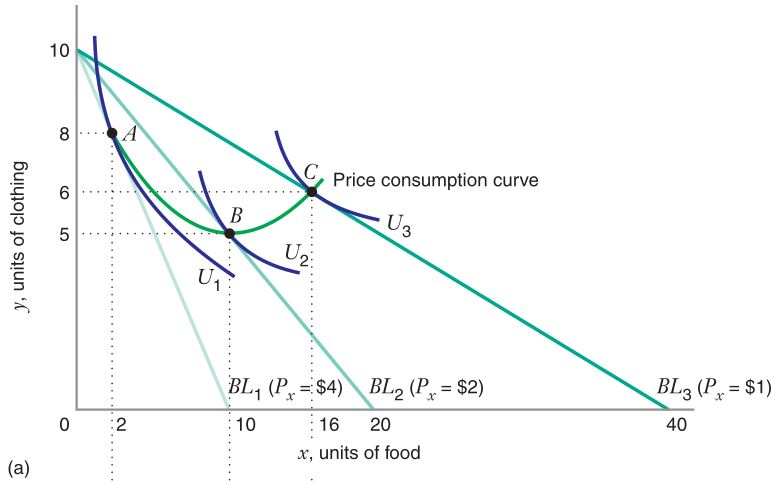
\includegraphics[width=240px]{figures/fig5_1a.jpg}
\end{figure}
\end{frame}

\begin{frame}{Optimal Choice and Demand}
These optimal bundles also map out the consumer's demand curve for good $x$.
\begin{figure}
  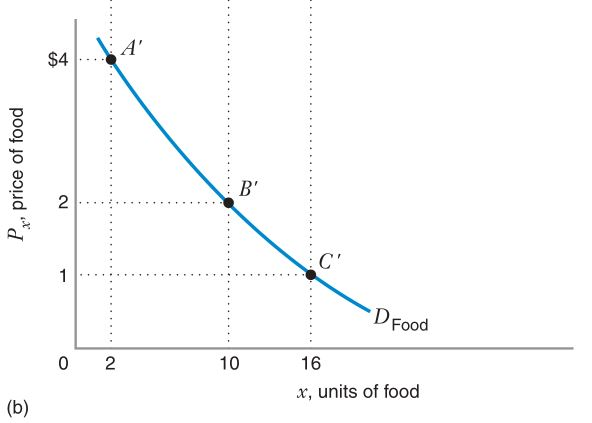
\includegraphics[width=220px]{figures/fig5_1b.jpg}
\end{figure}
\end{frame}

\begin{frame}{Optimal Choice and Demand}
  Note that as we move further \textit{along} the demand curve (i.e. as price falls), we reach higher and higher indifference curves.


  \bigskip\pause
  Remember that the demand curve represents a consumer's \textbf{willingness to pay} for a good. Two ways to think about the demand curve:

  \bigskip
  \begin{enumerate}
    \item A consumer's demand curve tells us how much the consumer is willing to pay \emph{for a given quantity}.

    \item  A consumer's demand curve tells us how much the consumer is willing to purchase \emph{for a given price}.
  \end{enumerate}
\end{frame}

\begin{frame}{Optimal Choice and Demand}
  What about a change in income?
  \begin{itemize}
    \item We can also map out (in a similar way to the price-consumption curve) what happens to a consumer's demand when their \emph{income} changes.

    \item This is called an \textbf{income consumption curve}.
  \end{itemize}
\end{frame}

\begin{frame}{Optimal Choice and Demand}
Below is the set of optimal bundles corresponding to various income levels. The connecting line is the \textbf{income consumption curve}.
\begin{figure}
  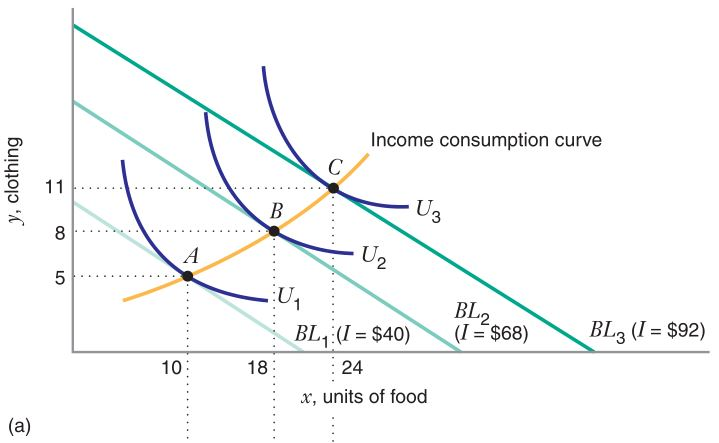
\includegraphics[width=230px]{figures/fig5_2a.jpg}
\end{figure}
\end{frame}

\begin{frame}{Optimal Choice and Demand}
  Remember that as income increases, the slope of the budget line doesn't change. 

  \begin{itemize}
    \item Ratio of prices stays the same!
  \end{itemize}

  \bigskip\pause
  The optimal bundles derived from various income levels can be used to map out \textit{shifts} of the demand curve (as in the following graph).
  
  \begin{itemize}
    \item The income consumption curve is \textit{not always} upward sloping (e.g. stop buying ramen as your income grows)
  \end{itemize}
\end{frame}

\begin{frame}{Optimal Choice and Demand}
  Below you can see how changes in income lead to shifts in the demand curve.

  \bigskip
  \begin{figure}
    \begin{tikzpicture}
      \begin{axis}[
        width = 10cm,
        height = 6cm,
        xmin = 0, xmax = 36,
        ymin = 0, ymax = 3,
        axis lines = left,
        xtick = {0, 10, 18, 24}, 
        ytick = {2},
        x label style={at={(axis description cs:0.5, -0.07)},anchor=north},
        y label style={at={(axis description cs:-0.07, .5)},anchor=south},
        xlabel = {\small $x$, units of food},
        ylabel = {\small $P_x$, price of food \$},
        clip = false,
      ]

        \addplot[alice!40,  very thick, smooth] plot coordinates 
          { (8, 2.6) (10, 2) (15, 1) (19, 0.55) };
        \addplot[alice!70,  very thick, smooth] plot coordinates 
          { (16, 2.75) (18, 2) (23, 1) (26, 0.6) };
        \addplot[alice!100, very thick, smooth] plot coordinates 
          { (22, 2.9) (24, 2) (28.5, 1) (31, 0.7) };

        % Points
        \addplot[color = black, dotted, thick] 
          coordinates {(0,2) (36, 2)}; 

        \addplot[color = black, dotted, thick] 
          coordinates {(10, 0) (10, 3)};   
        \node [anchor = south west] at (axis cs: 10, 2) 
          {\footnotesize $A''$};
        \addplot[color = black, mark = *, only marks, mark size = 2pt] 
          coordinates {(10, 2)};

        \addplot[color = black, dotted, thick] 
          coordinates {(18, 0) (18, 3)};
        \node [anchor = south west] at (axis cs: 18, 2) 
          {\footnotesize $B''$};
        \addplot[color = black, mark = *, only marks, mark size = 2pt] 
          coordinates {(18, 2)};

        \addplot[color = black, dotted, thick] 
          coordinates {(24, 0) (24, 3)};
        \node [anchor = south west] at (axis cs: 24, 2) 
          {\footnotesize $C''$};
        \addplot[color = black, mark = *, only marks, mark size = 2pt] 
          coordinates {(24, 2)};


        % Label Demand Curves
        \node [anchor = south, xshift=-0.2cm] at (axis cs: 8, 2.6) 
          [fill=white, text=alice!40, minimum size=0.5cm]{\footnotesize $D_1 \ (I = \$40)$};
        \node [anchor = south, xshift=-0.1cm] at (axis cs: 16, 2.75) 
          [fill=white, text=alice!70, minimum size=0.5cm]{\footnotesize $D_2 \ (I = \$68)$};
        \node [anchor = south, xshift=0.5cm] at (axis cs: 22, 2.9) 
          [fill=white, text=alice!100, minimum size=0.5cm]{\footnotesize $D_3 \ (I = \$92)$};
      \end{axis}
    \end{tikzpicture}
  \end{figure}
\end{frame}

\begin{frame}{Engel Curves}
  Another way of showing how a consumer's demand for a particular good varies with income is to draw an \textbf{Engel curve} which relates quantity demanded to income

  \bigskip
  \begin{figure}
    \begin{tikzpicture}
      \begin{axis}[
        width = 10cm,
        height = 6cm,
        xmin = 0, xmax = 36,
        ymin = 0, ymax = 130,
        axis lines = left,
        xtick = {0, 10, 18, 24}, 
        ytick = {40, 68, 92},
        x label style={at={(axis description cs:0.5, -0.07)},anchor=north},
        y label style={at={(axis description cs:-0.07, .5)},anchor=south},
        xlabel = {\small $x$, units of food},
        ylabel = {\small $I$, weekly income \$},
        clip = false,
      ]

        \addplot[black, very thick, smooth] plot coordinates 
          { (8, 36) (10, 40) (18, 68) (24, 92) (26, 104) };

        % Label Engel Curve
        \node [anchor = south west] at (axis cs: 26, 104) 
          {Engel Curve};

        % Points
        \addplot[color = black, dotted, thick] 
          coordinates {(0, 40) (10, 40) (10, 0)};   
        \node [anchor = south] at (axis cs: 10, 40) 
          {\footnotesize $A''$};
        \addplot[color = alice!40, mark = *, only marks, mark size = 2pt] 
          coordinates {(10, 40)};

        \addplot[color = black, dotted, thick] 
          coordinates {(0, 68) (18, 68) (18, 0)};   
        \node [anchor = south] at (axis cs: 18, 68) 
          {\footnotesize $B''$};
        \addplot[color = alice!70, mark = *, only marks, mark size = 2pt] 
          coordinates {(18, 68)};

        \addplot[color = black, dotted, thick] 
          coordinates {(0, 92) (24, 92) (24, 0)};   
        \node [anchor = south] at (axis cs: 24, 92) 
          {\footnotesize $C''$};
        \addplot[color = alice!100, mark = *, only marks, mark size = 2pt] 
          coordinates {(24, 92)};
      
      \end{axis}
    \end{tikzpicture}
  \end{figure}
\end{frame}

\begin{frame}{Engel Curves}
  If a consumer's Engel curve for a good is upward sloping (i.e. if as income rises, their consumption of the good increases), then the good is a \textbf{normal good}.

  \bigskip
  If the opposite is true, then the good is an \textbf{inferior good}.

  \bigskip\pause
  \begin{itemize}
    \item It is possible for a good to be a normal good over some interval, and an inferior good over another interval.

    \item What are some examples of normal and inferior goods?
  \end{itemize}
\end{frame}

\begin{frame}{Engel Curves}
In this example, hot dogs are a normal good when the consumer's income is lower, and an inferior good once their income is higher.
\begin{figure}
  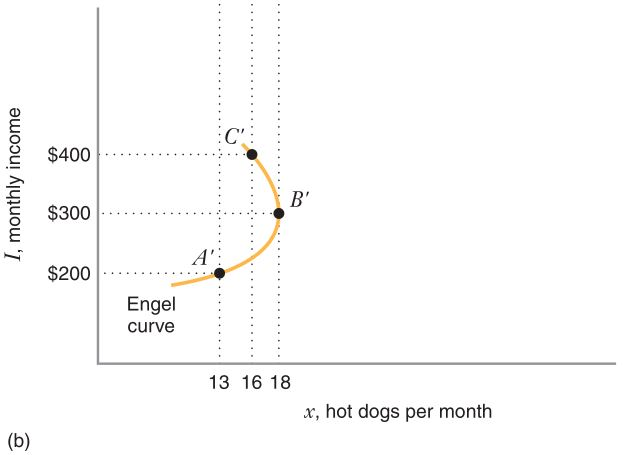
\includegraphics[width=220px]{figures/fig5_4b.jpg}
\end{figure}
\end{frame}

\begin{frame}
  \bgCoral{Try It Yourself} 

  \bigskip 
  Which of the following product demand functions indicates that the good is an \textbf{inferior} good?

  \bigskip
  \begin{enumerate}[A)]
    \item $x^*(p_x, I) = 2\frac{I}{P_x}$
    \item $x^*(p_x, I) =  2*I*P_x$ 
    \item $x^*(p_x, I) =  2*I*(10-P_x)$
    \item $x^*(p_x, I) =  2\big(\frac{40-I}{P_x}\big)$
  \end{enumerate}
\end{frame}

\begin{frame}{Substitution and Income Effects}
  Previously, we looked at the overall effect of changes in prices and income on demand for two goods.

  Here we will break that overall effect into two parts:

  \begin{enumerate}
    \item One due to the change in marginal utility per dollar of the affected good $MU_x / p_x$ 
    
    \item The other due to the fact that that $I / p_x$ increases
  \end{enumerate}
  
\end{frame}

\begin{frame}{Substitution and Income Effects}
  \begin{enumerate}
    \item The \textbf{substitution effect} refers to the change in demand caused by a change in the relative prices of two goods.

    \item The \textbf{income effect} refers to the change in demand for a good caused by a change in the consumer's  \textit{purchasing power} due to the price change.
  \end{enumerate}
\end{frame}

\begin{frame}{Substitution and Income Effects}
  Consider a case where the price of good $x$ decreases
  
  \bigskip
  \textbf{Substitution Effect}
  
  At the original bundle, $MU_x/p_x$ is now greater than $MU_y/p_y$ (since before the price changes, the two were equal)

  \smallskip
  You can now reach the same level of utility for less money by buying less of $y$ and more of $x$. This is the \textbf{substition effect}

  \bigskip
  \textbf{Income Effect}
  
  The \textbf{substitution effect} told use we reached the original utility for less money. So we have money left to spend. 
  
  \smallskip
  The additional consumption is the \textbf{income effect}!
\end{frame}

\begin{frame}{Substitution and Income Effects}
  On the following slides, we will look at how to graphically decompose a price change into income and substitution effects.
  \begin{figure}
    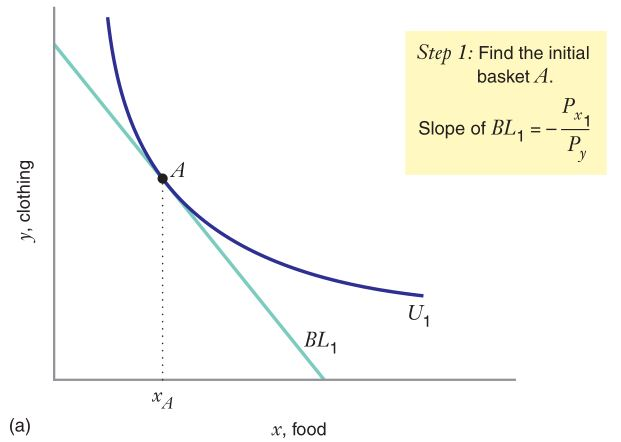
\includegraphics[width=240px]{figures/fig5_6a.jpg}
  \end{figure}
\end{frame}

\begin{frame}{Substitution and Income Effects}
  \begin{figure}
    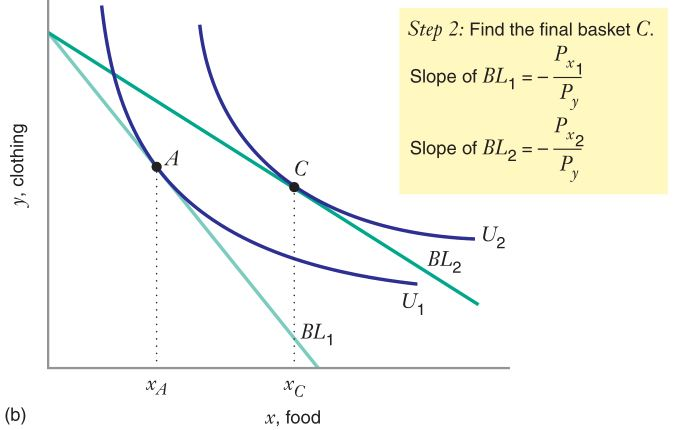
\includegraphics[width=240px]{figures/fig5_6b.jpg}
  \end{figure}
\end{frame}

\begin{frame}{Substitution and Income Effects}
  \begin{figure}
    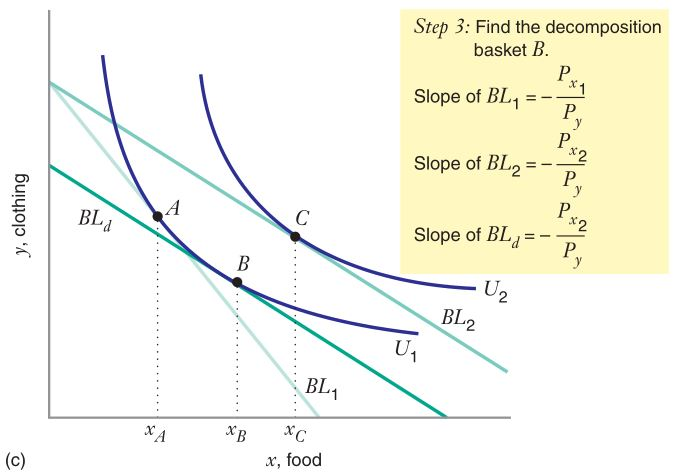
\includegraphics[width=220px]{figures/fig5_6c.jpg}
  \end{figure}

  \emph{Notice that in this case, the income effect leads to an increase in consumption of good x. That is, food is a normal good.}
\end{frame}

\begin{frame}{Substitution and Income Effects}
  \begin{figure}
    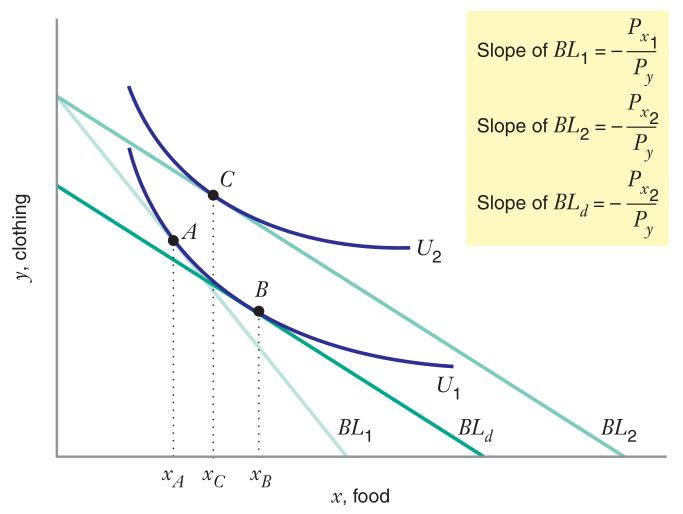
\includegraphics[width=220px]{figures/fig5_8.jpg}
  \end{figure}

  \emph{This is a case where food is an inferior good. The income effect leads to a decrease in consumption of good x.}
\end{frame}

\begin{frame}{Substitution and Income Effects}
  For both normal and inferior goods, the overall effect of an increase in price is a decrease in demand.

  \bigskip
  \begin{itemize}
    \item For normal goods, both the income and the substitution effects are negative.

    \item For inferior goods, the income effect is positive, but the substitution effect is negative, and the overall effect is negative.
  \end{itemize}
\end{frame}

\begin{frame}
  \bgCoral{Try It Yourself}

  \bigskip
  Suppose that peanut butter is an inferior good for many people. 
  
  \smallskip
  If the price increases, then would we expect demand for good $x$ to increase or decrease as a result of the substitution effect? What about due to the income effect?

  \bigskip
  \begin{enumerate}[A)]
    \item Increase, increase
    \item Increase, decrease
    \item Decrease, increase
    \item Decrease, decrease
  \end{enumerate}
\end{frame}

\begin{frame}{Estimating Changes in Consumer Welfare}
  Suppose the government wants to impose a tax on fast food. How can we measure the impact on consumer welfare?

  \begin{itemize}
    \item As we've talked about, we are not able to measure utility directly.

    \item But maybe we can measure changes to consumer wellbeing in monetary terms.

    \item We can do this in a few different ways.
  \end{itemize}
\end{frame}

\begin{frame}{Consumer Surplus}
  \textbf{Consumer Surplus} is the difference between the maximum amount that a consumer is \emph{willing to pay} for a good and the amount they must \emph{actually pay} in the marketplace.
  

  \bigskip\pause
  For example, suppose you want to buy a new pair of Nike running shoes. You would be willing to pay up to \$120 for them, but they are on sale for \$80. 

  \begin{itemize}
    \item Your consumer surplus if you buy the shoes is \$40.
    
    \item If the government then imposed a tax on Nike shoes, such that the price consumers pay increased by \$15, then your consumer surplus will decrease by \$15.
  \end{itemize}
\end{frame}

\begin{frame}{Consumer Surplus}
  Graphically, consumer surplus is calculated as the area below the demand curve and above the market price.

  \begin{figure}
    \begin{tikzpicture}
      \begin{axis}[
        width = 10cm,
        height = 6cm,
        xmin = 0, xmax = 45,
        ymin = 0, ymax = 12,
        axis lines = left,
        xtick = {0, 32, 40}, 
        ytick = {2, 10},
        x label style={at={(axis description cs:0.5, -0.07)},anchor=north},
        y label style={at={(axis description cs:-0.07, .5)},anchor=south},
        xlabel = {\small $Q$, gallons of milk},
        ylabel = {\small $P$, price of milk \$},
        clip = false,
      ]
        % Consumer Surplus
        \fill[kelly, opacity = 0.3] (0, 10) -- (32, 2) -- (0, 2) -- (0, 10);

        % Budget Line 1
        \addplot[domain = 0:40, samples = 400, color = cranberry, thick]{10 - 1/4*x};
        \node [anchor = south west] at (axis cs:40, 0) {$D_{\text{Milk}}$};

        % Demand Equation
        \node [anchor = south west] at (axis cs: 20, 7) 
          {$D_{\text{Milk}}: \ Q = 40 - 4P$};

        % Equilibrium
        \addplot[color = black, dotted, thick] 
          coordinates {(0, 2) (32, 2) (32, 0)};        
      \end{axis}
    \end{tikzpicture}
  \end{figure}
\end{frame}

\begin{frame}{Consumer Surplus}
  Suppose that you know the demand function for some market. In order to find the consumer surplus: 

  \begin{enumerate}
    \item First, plot the demand function

    \item Then, calculate the area of the triangle created by the market price and the demand curve.
  \end{enumerate}
\end{frame}

\begin{frame}{}
  \begin{figure}
    \begin{tikzpicture}
      \begin{axis}[
        width = 10cm,
        height = 6cm,
        xmin = 0, xmax = 45,
        ymin = 0, ymax = 12,
        axis lines = left,
        xtick = {0, 32, 40}, 
        ytick = {2, 10},
        x label style={at={(axis description cs:0.5, -0.07)},anchor=north},
        y label style={at={(axis description cs:-0.07, .5)},anchor=south},
        xlabel = {\small $Q$, gallons of milk},
        ylabel = {\small $P$, price of milk \$},
        clip = false,
      ]
        % Consumer Surplus
        \fill[kelly, opacity = 0.3] (0, 10) -- (28,3) -- (0, 3) -- (0, 10);
        \fill[ruby, opacity = 0.3] (0, 3) -- (28, 3) -- (28, 2) -- (0, 2) -- (0, 3);
        \fill[daisy, opacity = 0.3] (28, 3) -- (32, 2) -- (28, 2) -- (28, 3);

        % Budget Line 1
        \addplot[domain = 0:40, samples = 400, color = cranberry, thick]{10 - 1/4*x};
        \node [anchor = south west] at (axis cs:40, 0) {$D_{\text{Milk}}$};

        % Demand Equation
        \node [anchor = south west] at (axis cs: 20, 7) 
          {$D_{\text{Milk}}: \ Q = 40 - 4P$};

        % Equilibriums
        \addplot[color = black, dotted, thick] 
          coordinates {(0, 2) (32, 2) (32, 0)}; 
        \addplot[color = black, dotted, thick] 
          coordinates {(0, 3) (28, 3) (28, 0)};        
      \end{axis}
    \end{tikzpicture}
  \end{figure}

  When you increase the price, the consumer surpluse goes down for two reasons: 
  \begin{itemize}
    \item First, people who just barely bought no longer buy items
    
    \item Second, people that still buy after the price change have to pay more
  \end{itemize}
\end{frame}


\begin{frame}
  \bgCoral{Try It Yourself}
  
  \bigskip
  Suppose that consumer demand for organic, gluten-free dog food in Boulder can be represented by the following equation: $Q_D = 80 - 5P$. 
  
  \smallskip
  If the price of organic, gluten-free dog food is \$10 per pound, what is the consumer surplus?
\end{frame}

\begin{frame}
\end{frame}

\begin{frame}
  \bgCoral{Try It Yourself}
  
  \bigskip
  Suppose that consumer demand for organic, gluten-free dog food in Boulder can be represented by the following equation: $Q_D = 80 - 5P$. 
  
  \smallskip
  If the price of organic, gluten-free dog food increases to \$12 per pound (from \$10), what is the decrease in consumer surplus?
\end{frame}

\begin{frame}
\end{frame}

\begin{frame}{Compensating and Equivalent Variation}
  When considering the effects of price changes, we have two additional measures that may be useful: compensating variation and equivalent variation.

  \bigskip\pause
  \textbf{Compensating variation (CV)} measures how much a consumer's income would have to change to keep them at the \textbf{same} utility level as before a price change, \textbf{after} the price change has occurred.
  
  \begin{itemize}
    \item For example, suppose that the government wants to impose a tax on Nike shoes.
    
    \item CV tells us how much the government would have to compensate consumers to make up for the decreased wellbeing caused by the price increase.
  \end{itemize}
\end{frame}

\begin{frame}{Compensating and Equivalent Variation}
  \textbf{Equivalent variation (EV)} measures how much a consumer's income would have to change \textbf{before} a price change has occurred to make them indifferent between the price change and the additional income.

  \begin{itemize}
    \item For example, suppose the government announces a tax break on home purchases (essentially lowering the price of houses), but then decides to instead just give taxpayers an income tax credit instead.

    \item EV measures how much of an income tax credit taxpayers would have to receive to be indifferent between the proposed home tax break and the income tax credit.

    \item Note that, unlike the CV example, the price change \textbf{has not} actually occurred.
  \end{itemize}
\end{frame}

\begin{frame}{Compensating and Equivalent Variation}
  Here's another way to remember the difference between EV and CV:
  
  \bigskip
  \begin{itemize}
    \item Compensating variation measures the income that would be needed to \textbf{compensate} the consumer for a price change.

    \item Equivalent variation measures the income change that would be \textbf{equivalent} to a hypothetical or proposed price change.
  \end{itemize}
\end{frame}

\begin{frame}{Compensating and Equivalent Variation}
  Below is a graphical representation of EV and CV.
  \begin{figure}
    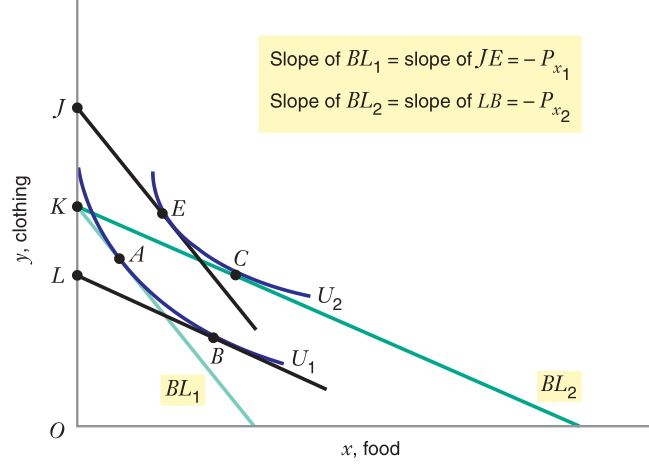
\includegraphics[width=240px]{figures/fig5_15.jpg}
  \end{figure}
\end{frame}


\begin{frame}{Compensating and Equivalent Variation}
  Note that CV and EV are often not the same.
  
  \bigskip
  \begin{itemize}
    \item This is due to income effects.

    \item EV measures income needed to get to the new level of utility at \textbf{old} prices, and CV measures income needed to get back to the original utility level at \textbf{new} prices.
  \end{itemize}
\end{frame}

\begin{frame}{Compensating and Equivalent Variation}
  Which measure you should use depends on the situation:

  \bigskip
  \begin{itemize}
    \item If the government wants to impose a larger tax on marijuana to reduce consumption, but doesn't want people to be worse off, CV is appropriate.

    \item If the government promised a subsidy on electric vehicles, and then decided to give income tax credits instead, EV is appropriate.
  \end{itemize}
\end{frame}

\begin{frame}
  \bgCoral{Try It Yourself}
  
  \bigskip
  Suppose that a private company offered it's workers an employee discount on all products, but then later decided to instead increase their wages. They want to know how much the need to increase wages by to make people as well off as the proposed discount would have. Should you use the Compensating Variation or the Equivalent Variation?
\end{frame}

\begin{frame}{The Labor-Leisure Decision}
  One decision that almost every individual must make is whether to work, and how much. Economists refer to this as the \textbf{labor-leisure decision}. 

  \bigskip
  \begin{itemize}
    \item Leisure refers to all nonwork activies, such as eating, sleeping, recreation, and entertainment.

    \item Many people would love to allocate \textbf{all} of their time toward leisure.

    \item But why can't they?
  \end{itemize}
\end{frame}

\begin{frame}{The Labor-Leisure Decision}
  A consumer has to earn money to spend it on goods. So she must give up some leisure in order to earn money.

  \bigskip
  A consumer has $24$ hours in a day. She spends $L$ of those on leisure activies, and $(24 - L)$ on labor activities. Suppose her wage is $w$
  
  \bigskip
  \begin{itemize}
    \item Then her daily income is therefore $w(24-L)$ 

    \item This can use to buy a composite good at a price of $\$1$.
  \end{itemize}
\end{frame}

\begin{frame}{The Labor-Leisure Decision}
  The consumer's budget contraint can be written as
  $$
    Y = w (24 - L)
  $$

  \bigskip
  We can also rearrange that, so that it looks more like our typical budget constraint.
  $$
    24w = wL + Y
  $$
\end{frame}

\begin{frame}{The Labor-Leisure Decision}
  $$
    24w = wL + Y
  $$

  Written this way, we can think of it in more conventional terms.
  \bigskip
  \begin{itemize}
    \item We can think of her income as $24w$.

    \item She can spend her income on leisure (at a 'price' of w, her wage).

    \item And she can spend it on the composite good.

    \item Her utility $U$ depends on the amount of leisure time she has, and on how much of the composite good she can buy.
  \end{itemize}
\end{frame}

\begin{frame}{The Labor-Leisure Decision}
  Below is an illustration of the budget lines and optimal leisure-composite good bundles for a consumer at various wages.

  \begin{figure}
    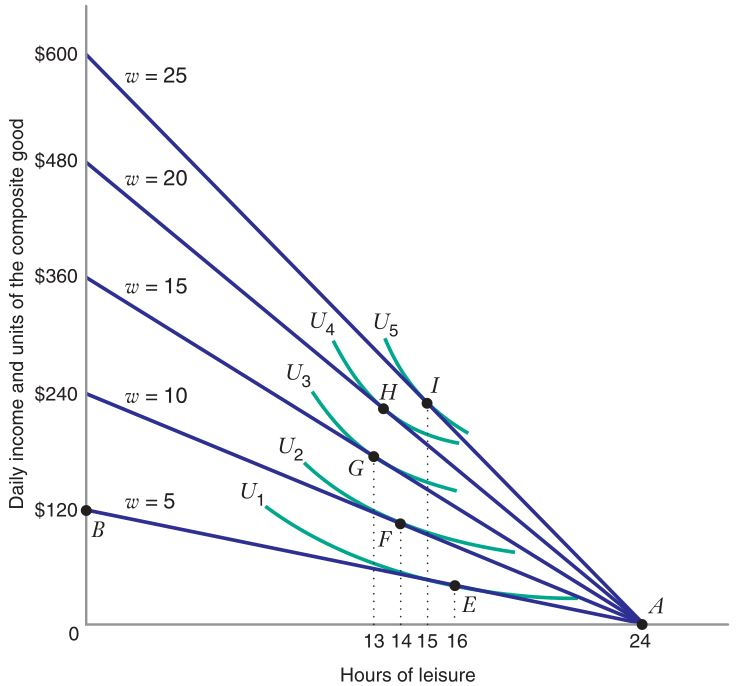
\includegraphics[width=170px]{figures/fig5_24.jpg}
  \end{figure}
\end{frame}

\begin{frame}{The Labor-Leisure Decision}
  Let's consider the \coral{trade-off} at play here:
  
  \begin{itemize}
    \item If the consumer spends all of their time on leisure, they will earn no money and have nothing to spend on the composite good.

    \item On the other hand, if they work, they can buy more stuff
  \end{itemize}
\end{frame}

\begin{frame}{The Labor-Leisure Decision}
  In general, we assume that the consumer's labor supply curve (the curve tracing out all of the optimal bundles for various wages) is backward bending.
  
  \bigskip
  \begin{itemize}
    \item That is, as their wage increases, they works more up to a certain point.

    \item Beyond that, as their wage increases they works less.

    \item This again relates to the \textit{income} and \textit{substitution} effects on labor supply.
  \end{itemize}
\end{frame}

\begin{frame}{The Labor-Leisure Decision}
  Below is a backward-bending supply curve. At low wages, an increase in the wage results in a greater supply of labor. But eventually, supply diminishes as the wage rises.

  \begin{figure}
    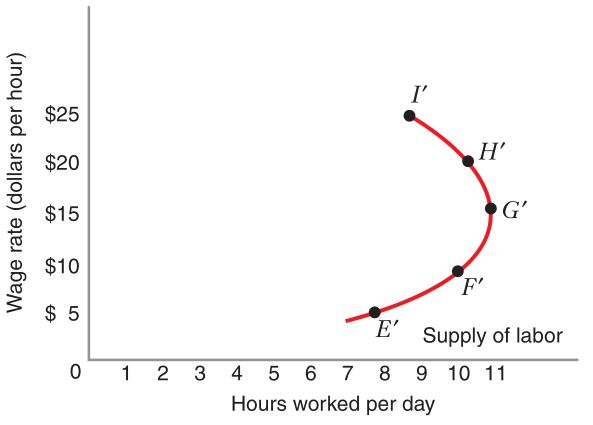
\includegraphics[width=220px]{figures/fig5_25.jpg}
  \end{figure}
\end{frame}

\begin{frame}{The Labor-Leisure Decision}
  In this model, the substitution effect is negative;
  
  \bigskip
  \begin{itemize}
    \item As the wage increases, the opportunity cost of an hour of leisure, $w$, increases, and leisure becomes more 'expensive'.

    \item So the worker will substitute some leisure for more of the composite good.
  \end{itemize}
  
  \bigskip\pause
  The income effect is positive.

  \bigskip
  \begin{itemize}
    \item As a consumer's wage increases, their income increases, so they 'buy' more leisure (because leisure is a normal good).
  \end{itemize}
\end{frame}

\begin{frame}{The Labor-Leisure Decision}
  Initially, the substitution effect dominates. As the wage rises, people work more.
  
  \bigskip 
  But eventually, the income effect dominates. As the wage rises, people work less
\end{frame}

\begin{frame}
  \bgCoral{Try It Yourself}
  
  \bigskip
  Suppose that a worker in the U.S initially earns \$10/hour. Then, due to company-wide pay cuts, the worker is given a pay cut of \$1.50/hour, and as a result, decides to work more. The worker's decision to work more implies that which effect (the income or substitution effect) is dominating?
\end{frame}

\begin{frame}{Conclusion}
  This wraps up the content on consumer theory.

  \bigskip
  \begin{itemize}
    \item We discussed how consumers rank various bundles of goods.

    \item  And how consumers make decisions in a variety of contexts.

    \item We've also discussed how consumer welfare, and changes in it, can be measured.
  \end{itemize}
\end{frame}

\end{document}
